\subsection{Tools and Languages}

We have implemented \thename{} in the C Programming Language, more specifically
using the C99 standard with GNU extensions by use of GCC~\cite{gnu:gcc}. There
are both pros and cons of using a relatively low-level language (as compared to
other available languages), but we found that the benefits outweighed the
disadvantages.

First of all C is extremely portable; GCC is available on \textit{a lot} of
architectures, and all modern operating systems ship with a C compiler which
essentially is all that is required to build \thename{} for a new platform. The
standard libraries and architecture specific functions available differ with
each machine and device, so we aim at relying on as few external libraries as
possible and provide wrappers for the ones we use so that the implementation can
be ported easily.

Secondly we do not want to rely on a garbage collector provided by languages
like C++ and Java. We need full control over where each bit of data is stored,
mostly for performance reasons both in terms of memory footprint and execution
speed.

Third, speed is of the essence and C is notoriously fast, given that the code is
well-written.

There are however downsides to using C. Because we are not veterans of C and due
to its low-level nature it is inherently more difficult to develop features that
could be implemented in a few lines of code in a higher-level language, and
memory has to be tracked meticulously to prevent memory leaks. We have found
that it is a great exercise for becoming proficient with programming in general
because it provides us with knowledge of the mechanisms that lie behind concepts
that are generally taken for granted.

\textbf{Note:} The code snippets presented in the following sections do not
always correspond directly with the code found in the actual
implementation. They carry the gist of what we want to communicate but generally
avoids unnecessary and redundant information not relevant to the individual
cases.

\subsection{Code Style}

The C languages liberates the programmer to structure code and data in about as
many ways as one can imagine. This can be both a blessing and a curse, and
warrants some agreed upon conventions to maintain consistency.

For a module of functionality we use a general pattern that consists of a struct
containing the state or data of a piece of machinery, and corresponding prefixed
functions that take such a structure as argument and operate on its
data. Stacks, for instance, are implemented with a \code{stack} struct, and the
functions \code{stack\_init}, \code{stack\_pop}, \code{stack\_free}, etc. This
essentially mimics object orientation from other languages (C++, Java), but has
the benefit of most functions being \term{pure}, i.e.~a function that only
depends on its input, making testing and reasoning about the code easier.

\subsection{Core Infrastructure}
\label{sec:implementation:core}

The infrastructure of \thename{} is the code that lays the basis for interaction
between the individual parts of the system. It is a collection of machinery
which hand control back and forth between each other, such as the instruction
cycle, thread management and exception handling. Besides the machine's exposed
exception handling system there is an internal error handling system which
allows errors within the machine to be handled as gracefully possible.

The implementation of the machine is divided into several modules each of which
serve a specific purpose. Figure~\ref{fig:implementation:arch} shows the
overarching architecture and which modules depend on each other.

The \textit{Engine} module is the top-most control unit that is used to set
everything in motion. It only implements two functions; \code{start} which
initializes the other components and begins execution, and \code{stop} that
frees the resources claimed by the machine and exits gracefully. The
\textit{Abstract Machine} module is responsible for reading the byte code,
parsing it into opcodes, instruction prefixes and argument values and
subsequently delegating the work to the \textit{Instruction Executer}. That is
where the guts of the system lies and where all program logic is performed. It
manipulates the stack through the \textit{Stack} module which implements the
data structures and exposes an interface for pushing, popping, replacing and
peeking into those. The \textit{Information Tables} modules is really three
modules, one for each of the string, constant and metadata table which are all
interfaces to global tables with functions to look up entries by various
criteria. The \textit{Garbage Collector} is the interface to the memory managing
unit, and is responsible for allocating memory on the heap and automatically
releasing it when it is no longer in use. Finally, the \textit{Thread} module
handles creation and destruction of threads in which all program code is
executed.

\begin{figure}
  \centering
  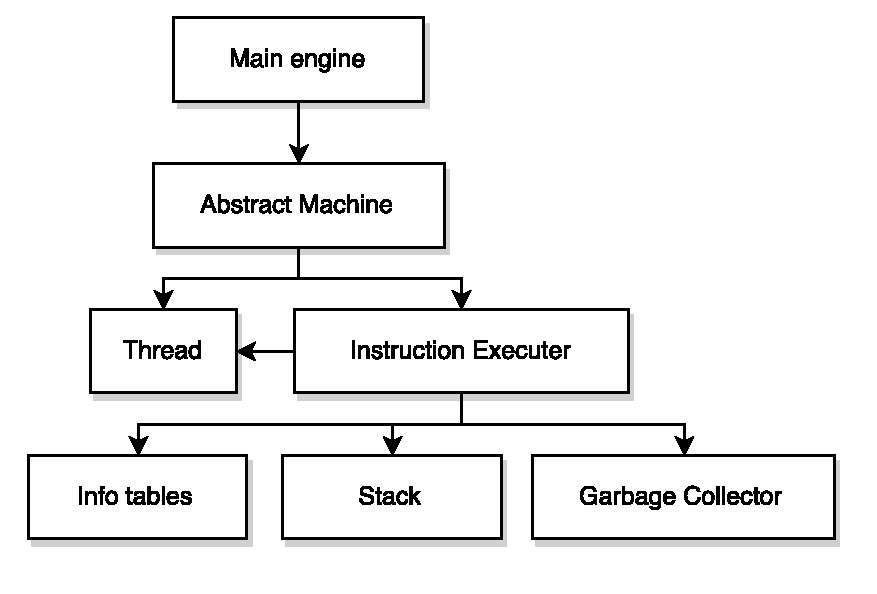
\includegraphics[width=0.6\textwidth]{figures/arch}
  \caption{The architecture of \thename{}. An arrow represents a dependency
    where the module pointed \emph{from} depends on the module pointed
    \emph{to}.}
  \label{fig:implementation:arch}
\end{figure}

During the initialization phase the machine carries out approximately the
following steps:

\begin{enumerate}
\item Parse command-line arguments
\item Set up internal error handling mechanisms
\item Initialize the global abstract machine state
\item Parse the input executable file
  \begin{enumerate}
  \item Load byte code from the executable
  \item Load information tables (not implemented)
  \end{enumerate}
\item Initialize scope
  \begin{enumerate}
  \item Create an implicit root scope, ancestor to all future scopes
  \item Load the the run-time library functions into the root scope
  \end{enumerate}
\item Initialize main thread
  \begin{enumerate}
  \item Allocate a thread
  \item Allocate a stack for it
  \end{enumerate}
\item Begin the instruction cycle in the main thread
\end{enumerate}

The following sections details how the above steps are performed.

\subsubsection{Command-line Arguments}
The common way, and arguably the only way the makes sense, of customizing the
parameters of an executable is through command-line arguments, given directly to
the executable when run. These arguments can be extended to do a number of
things, but essentially we only require the name of the binary file to be
executed and optionally customizing the level of verbosity, i.e. the amount of
logging information to display. %TODO første del lidt derp? watfix?

The input file is set with the {\tt --file} (or {\tt -f}) argument, and the
verbosity level is set with either {\tt --brief} ({\tt -b}) or {\tt--versbose}
({\tt -v}). For more information on logging, see
section~\ref{sec:implementation:core:debug} below.

We follow common conventions by having two special arguments for displaying
useful meta information about the \thename{} binary. These include the {\tt
  --help} argument for printing information on the different arguments, and {\tt
  --version}, for simply printing the version of the binary.

For ease of implementation we use the Getopt library~\footnote{Getopt (libc):
  \url{http://www.gnu.org/software/libc/manual/html_node/Getopt.html}}, included
in C's Standard Library.

\subsubsection{Internal Error Handling}

When writing software, history has shown that bugs are unavoidable, and we do
not expect \thename{} to be an exception. Rather than denying this fact, we try
to remedy the situation by gracefully exiting the program, while also trying to
give some useful information about what went wrong. This makes it easier for
users to understand what is going on and reporting the problem so it can fixed.

Internal errors can occur in two ways. Either by the machine checking the value
of different parameters, ensuring they are of the expected format, and if they
are not we can cowardly stop the machine without crashing. The other scenario is
an error occuring by the operating system signaling the machine that it is
trying to do something illegal. In this we can catch the signal, which follows
the POSIX-standard, and again gracefully exit the program.

When we say gracefully exit, we mean that we can stop running threads, free any
allocated memory, print some information and set the return code of the
process. The two last things are very important to let the user know what has
happened, but also to debug the problem.

Errors can be invoked through a special logging macro {\tt log\_err}, described
in the \nameref{sec:implementation:core:debug} section
below.

\subsubsection{ELF File Loading}

The first thing the machine does upon start up is to load the input file that is
going to be executed. The current implementation does not read information
tables which means that only the byte code is loaded. Information table entries
can be hardcoded into the system easily, which is what we have done for testing
purposes.

In the \code{loader} module, we use the library Libelf\footnote{libelf:
  \url{https://directory.fsf.org/wiki/Libelf}} to parse and extract data from
the input file. It provides the means to easily parse ELF files and search
through segments and sections, making the process of byte code loading quite
simple indeed. The file is verified to be a valid, parsable ELF file before
beginning any data extraction. Libelf exposes a function to get the section
following another by use of which the sections are iterated. We need to extract
the data of the \code{.text} section which is where the byte code is stored in
its entirety. Thus for each section we simply check its name and if it matches
we copy the bytes from the section into the abstract machine state's code field.

\subsubsection{Instruction Cycle}

The fundamental means of operation in the machine is the execution of
instructions that are parsed and interpreted from byte code. Each thread runs
their own cycle, the essence of which is shown in
Listing~\ref{lst:implementation:instruction-cycle}

\begin{lstlisting}[%
  caption={Pseudo representation of the instruction cycle},%
  label={lst:implementation:instruction-cycle}]
while (thread is running) {
  fetch opcode
  fetch potential arguments
  update program counter
  execute instruction corresponding to opcode
}
\end{lstlisting}

All instruction functions take a \code{thread\_state*} argument that they use to
manipulate the thread's stack, change the program counter, access scopes and so
on.

As an example consider the following byte code stream:

\code{0: 0xFC, 1: 0x04, 2: 0x00, 3: 0x00, 4: 0x05, 5: 0x39, ...}

And let the program counter be $pc = 0$. The machine will carry out the
following:

\begin{enumerate}
\item Read instruction prefixes
  \label{item:read-prefix}
  \begin{enumerate}
  \item Look for bytes that are valid prefix values which currently is any value
    greater than or equal to \code{0xFC} (decimal 252).
  \item The byte at $pc=0$, \code{0xFC}, is a valid prefix, namely the
    \code{large} prefix.
  \item Set the \code{pre\_large} flag in the executing thread's state and
    increment program count, $pc \leftarrow pc + 1 \Rightarrow pc= 1$
  \item The byte at $pc=1$, \code{0x04}, is not a valid prefix, thus stop
    reading prefixes.
  \end{enumerate}

\item Read the opcode which is always a single byte. The byte at $pc=1$ is
  \code{0x04} which corresponds to the \instr{pushConstant} instruction.

\item Increment program counter, $pc \leftarrow pc + 1 \Rightarrow pc = 2$

\item Fetch arguments
  \begin{enumerate}
  \item \instr{pushConstant} takes an argument, an integer value representing a
    constant table index.
  \item The \code{pre\_large} flag is true, so we must read the argument as a
    32-bit (four bytes) integer.
  \item Interpret the next four bytes as a big endian integral value. The four
    bytes are \code{0x00, 0x00, 0x05, 0x39} which is interpreted as the value
    \code{0x539} (decimal 1337).
  \item Increment program counter by four bytes,
    $pc \leftarrow pc + 4 \Rightarrow pc = 6$
  \end{enumerate}

\item Call the instruction function for \instr{pushConstant} with the argument
  $1337$.

\item Go to~\ref{item:read-prefix}.

\end{enumerate}

The implementation of concrete instructions is detailed in
Section~\ref{sec:implementation:instr}.

\subsubsection{Logging and Debugging}
\label{sec:implementation:core:debug}

\thename{} has a logging system, found in the {\tt logger.h} module. It handles
all messages sent by all components of the machine and decides whether to print
them to {\tt stdout}. This decision is based on a logging level, which is part
of the global state of the machine. The logging level sets the ``barrier'' for
when a message should be printed. The available levels includes {\tt brief},
{\tt normal} and {\tt verbose} which can be customized through command-line
arguments, but defaults to {\tt normal}. As each log message is also categorized
with a level of severity, the logging module compares the logging level and the
message level to decide whether the message should be printed. The message
levels are {\tt error}, {\tt warning} and {\tt info}.

If the logging level is set to brief, only warnings will be printed, if set to
normal, warnings will also be printed, and lastly, if set to verbose, everything
will be printed.

A log message is sent through an interface of macros, exposed by the {\tt
  logger.h} header-file. Each message level has two logging macros, logging a
message of the given severity level. The two macros include one which takes a
string, and a formatted version, suffixed with ``f'', which takes a formatted
string and a variable number of arguments (in the same fashion as
\code{printf}).

\begin{ccode}
#define log_warn(msg)                             \
  do {                                            \
      if (should_log(WARNING)) {                  \
          fprintf(stderr, "warning: " msg "\n");  \
      }                                           \
  } while (0)
\end{ccode}

The {\tt log\_err} macro, will in addition to logging an error message also
clean up and stop the machine, as it cannot safely continue. The message will be
printed to {\tt stderr} instead of {\tt stdout}, so the overlaying environment
running \thename{} can act accordingly.

For debugging during development there is two extra macros for printing a
message prefixed with file name, function name and line number. One of which is
suffixes with ``f'', denoting it takes a formatted string in the same manner as
the logging macros. The debug messages are only displayed if the {\tt DEBUG} macro value is
defined. This value is automatically set through the build system, for
convenience during development.

\subsection{Stacks}
\label{sec:implementation:stacks}
A stack is in itself a fairly simple construction that allows values to be
pushed to an popped from an allocated memory region. Stack elements are stored
and retrieved by the Last-In, First-Out (LIFO) principle.

\subsubsection{Stack elements}

Each element on a stack holds information about both the \textit{declared} and
\textit{actual} type of data that it contains. Details on this is described in
\ref{NEEDED}. The data part of a stack element is a simple array of bytes,
stored in big endian order, i.e.~the most significant bit is at the lowest
memory address.

\subsubsection{Memory Layout}

Arguably the most intuitive way to construct a stack is to use a simple array of
a fixed initial size and handle operations by keeping track of the number of
elements in the stack. A push operation would thus increments the number of
elements and assigns a value to the new top-most slot. A pop operation will
correspondingly decrement the number of elements in the stack and potentially
return the element that is being removed. When the number of elements in the
stack exceeds the initial size of the containing array more memory must be
allocated. This can be done simply by use of \code{realloc} where the common
approach is to double the amount of allocated memory, to adapt to quickly
growing stacks. However, \code{realloc} can be a performance issue because it
will create a new allocation, copy over the current data and free the old
allocation, in the case the there is no more space directly following what is
being reallocated~\cite{man-realloc}. This is arguably an expensive operation,
and since the stack is by far the most frequently used means of operation in
\thename{}, it is critical that it performs well.
% TODO: agree ^ realloc not _always_ moves memory, but etc?

An important thing to consider is that the content of a stack element depends on
the type of the element, and thus have varying sizes. An element whose type is
\code{Int8} requires a single byte for storage while an element of type
\code{Int32} requires 4 bytes of storage and static arrays can be arbitrarily
large. Since we do not want to waste memory on redundant bytes, that prevents us
from implementing stack elements as fixed size structures laid out in an array
as described above. We have solved the problem by implementing stack elements as
a singly linked list going from the top element down to the bottom. The memory
used by the stack should be as contiguous as possible, to avoid a large amount
of allocations and deallocations, and the elements in the linked list should
reside one after another in memory. The actual content of an element is stored
\textit{in between} the linked list nodes, and the \code{next} pointer simply
points to the memory address following its content data
bytes. Figure~\ref{fig:implementation:stack-layout} shows how the stack elements
are laid out, with arrows denoting pointers.

\begin{figure}[H]
  \centering
  \begin{drawstack}[every initial by arrow/.style={*->}]
  \startframe{}
  \cell{Declared type} \cellcom{\texttt{rtti*}} \coordinate (next) at (currentcell.east);
  \cell{Actual type} \cellcom{\texttt{rtti*}}
  \cell{Next} \cellcom{\texttt{stack\_element*}}
  \cell{Content size} \cellcom{\texttt{int}}
  \padding{2}{Content}  \cellcom{\texttt{char[]}}
  \finishframe{\texttt{stack\_element}}

  \startframe{}
  \cell{Declared type}  \cellcom{\texttt{rtti*}}
  \cell{Actual type}  \cellcom{\texttt{rtti*}}
  \cell{Next} \cellcom{\texttt{stack\_element*}} \coordinate (el2) at (currentcell.east);
  \cell{Content size} \cellcom{\texttt{int}}
  \padding{2}{Content}  \cellcom{\texttt{char[]}}
  \finishframe{\texttt{stack\_element}}
  \startframe{}

  \draw[->, thick, bend right=20] (el2) edge (next);
\end{drawstack}

% \begin{drawstack}
%   \startframe
%   %   \cellcom writes something on the right-hand side of a cell.
%   \cell{loc2} \cellcom{-8(\%ebp)}
%   \cell{loc1} \cellcom{-4(\%ebp)}
%   %   \esp and \ebp are stack pointer and base pointer in Pentium.
%   %   These macros are simple shortcuts for \cellptr{...}
%   \cell{Sauvegarde \%ebp} \esp \ebp
%   \cell{@ retour} \cellcom{4(\%ebp)}
%   \finishframe{fonction\\ {\tt f}}
%   \startframe
%   \cell{} \cellcom{8(\%ebp)}
%   \cell{}
%   \finishframe{fonction\\ {\tt main}}
% \end{drawstack}

% \section{Padding}

% \begin{drawstack}
%   \cell{above padding}
%   \padding{3}{nothing here}
%   \cell{below padding}
% \end{drawstack}

% \section{Below/Above stack pointer}

% \begin{drawstack}
%   \cell{Top}
%   \cell{Below top}
%   %   \bcell is just like \cell, but in a different color.
%   \bcell{Above bottom} \cellptr{Stack pointer here}
%   \bcell{Bottom}
% \end{drawstack}

% \section{Highlighting some cell}

% \begin{drawstack}
%   \cell{Uninteresting cell}
%   \cell{Interesting cell} \cellround{Yes, this one!}
% \end{drawstack}

% \section{Structures without a stack structure}

% \begin{tikzpicture}
%   \draw (3, -1) node (Otm) {
%   \begin{tabular}{c}
      %       Object\\vtable
      %     \end{tabular}
      %       };

      %       \drawstruct{(0,0)}
      %       \structcell[freecell]{~} \coordinate (Atm) at (currentcell.east);
      %       \structcell[freecell]{\texttt{@Object.equals()}}
      %       \structcell[freecell]{\texttt{@code A.m()}}
      %       \structcell[freecell]{\texttt{@code A.p()}} \coordinate (A) at (currentcell.west);
      %       \structname{
      %       \begin{tabular}{c}
      %       A's vtable
      %     \end{tabular}
      %       }

      %       \drawstruct{(-4,-3)}
      %       \structcell[freecell]{} \coordinate (Btm) at (currentcell.east);
      %       \structcell[freecell]{\texttt{@Object.equals()}}
      %       \structcell[freecell]{\texttt{@code A.m()}}
      %       \structcell[freecell]{\texttt{@code B.p()}}
      %       \structcell[freecell]{\texttt{@code B.q()}}
      %       \structname{B's vtable}

      %       \draw[->] (Btm) -- (A);
      %       \draw[->] (Atm) -- (Otm);
      %       \end{tikzpicture}

      %       \section{Structures and stack together}

      %       \begin{tikzpicture}[scale=.8]

      %       \stacktop{}
      %       \separator
      %       \cell{\texttt{p3}}        \cellcomL{11(GB)} \coordinate (p3) at (currentcell.east);
      %       \separator
      %       \cell{\texttt{p2}}        \cellcomL{10(GB)} \coordinate (p2) at (currentcell.east);
      %       \separator
      %       \cell{\texttt{p1}}        \cellcomL{ 9(GB)} \coordinate (p1) at (currentcell.east);
      %       \separator
      %       \cell{\texttt{@P3D.diag}} \cellcomL{ 8(GB)}
      %       \cell{\texttt{\footnotesize @Object.equals}} \cellcomL{ 7(GB)}
      %       \cell{\texttt{3(GB)}}     \cellcomL{ 6(GB)} \coordinate (T1) at (currentcell.east);
      %       \separator
      %       \cell{\texttt{@P2D.diag}} \cellcomL{ 5(GB)}
      %       \cell{\texttt{\footnotesize @Object.equals}} \cellcomL{ 4(GB)}
      %       \cell{\texttt{1(GB)}}     \cellcomL{ 3(GB)} \coordinate (T2) at (currentcell.east);
      %       \separator
      %       \cell{\texttt{\footnotesize @Object.equals}} \cellcomL{ 2(GB)}
      %       \cell{\texttt{null}}      \cellcomL{ 1(GB)}
      %       \cell[draw=none]{Stack}


      %       \drawstruct{(5,1)})
      %       \structcell{z=2,5}
      %       \structcell{y=2,5}
      %       \structcell{x=2,5}
      %       \structcell{.} \coordinate (O1) at (currentcell.west);
      %       \coordinate (O1l) at (currentcell.south);

      %       \drawstruct{(9,-3)}
      %       \structcell{y=1}
      %       \structcell{x=1}
      %       \structcell{.} \coordinate (O2) at (currentcell.west);
      %       \coordinate (O2l) at (currentcell.south);

      %       \draw[->] (p3) -- (O1);
      %       \draw[->] (p2) -- (O1);
      %       \draw[->] (p1) -- (O2);

      %       \draw[->] (O1l) .. controls (O1 |- T1) .. (T1);
      %       \draw[->] (O2l) .. controls (O2 |- T2) .. (T2);

      %       \draw (10,-10) node{Heap};

      %       \end{tikzpicture}



      %       \section{Using tikzpicture instead of drawstack}

      % %       The environment drawstack is basically a syntactic sugar for
      % %
      % %       \begin{tikzpicture}[#1]
      % %         \stacktop{}
      % %         ...
      % %         \stackbottom
      % %       \end{tikzpicture}
      % %
      % %       You can use the above syntax for more flexibility.

      %       \begin{tikzpicture}[scale=0.8]
      %       \small
      %       \stacktop{}
      %       \cell{My cell}
      %       \stackbottom{}
      %       \end{tikzpicture}

      %       \section{Changing style}

      %       {% tikzstyle will be local to this {...}
      %       \tikzstyle{freecell}=[fill=blue!10,draw=blue!30!black]
      %       \tikzstyle{occupiedcell}=[fill=blue!10!orange!10,draw=blue!30!black]
      %       \tikzstyle{padding}=[fill=yellow!20,draw=blue!30!black]
      %       \tikzstyle{highlight}=[draw=orange!50!black,text=orange!50!black]

      %       \begin{drawstack}
      %       \cell{Uninteresting cell}
      %       \cell{Interesting cell} \cellround{Yes, this one!}
      %       \bcell{bcell}
      %       \padding{2}{Padding}
      %       \end{drawstack}
      %       }

      %       \section{Example: Computing Factorial}

      %       \begin{drawstack}[scale=0.8]
      %       \startframe
      %       \cell{N = 1}
      %       \cell{...}
      %       \finishframe{fact(1)}
      %       \startframe
      %       \cell{N = 2}
      %       \cell{...}
      %       \finishframe{fact(2)}
      %       \cell{$\vdots$}
      %       \startframe
      %       \cell{N = 5}
      %       \cell{...}
      %       \finishframe{fact(5)}
      %       \end{drawstack}

  \caption{Stack memory layout}
  \label{fig:implementation:stack-layout}
\end{figure}

The C language does not support variable length arrays, which means that an
array must have its length declared, otherwise the type is regarded as
incomplete. However, line~\ref{code:stack-element:flexible-data} in
Listing~\ref{lst:implementation:stack:element} shows a feature known as a
\term{flexible array} that allows the last field of a struct to be declared as a
size-less array. We take advantage of exactly that so that we can easily
interpret the \code{data} field of an element as an array of bytes of any size.

What is left to solve is the problem of a stack growing beyond its initial
size. As mentioned, reallocation of the memory used by the stack works, but
results in poor performance. To mitigate the issue we have modelled the stack as
a linked list of allocated memory regions which we call \textit{segments}. Each
segment is essentially a stack in itself and is implemented exactly as described
above. The benefit is that when a segment becomes full, a new segment is simply
allocated and wired into the linked list, thus preventing the need for a
reallocation. The exposed interface of the stack consists of a set of stack
operation functions that essentially maps operations onto segments by selecting
the appropriate segment, and potentially what index of its elements that will be
the target of a given operation. Thus the segments are hidden in the
implementation and are solely internal data structures which users of the stack
are ignorant of.

\begin{remark}
  A segmented stack is not a novel idea. They are used by the Go programming
  language to facilitate large amounts of unbounded stacks (for concurrent
  sub-routines called goroutines). The Rust programming language did as well but
  later abandoned them. There are arguments for not using them because of the
  overhead generated by extra work needed when stack limits are
  exceeded\cite{rust:segmented-stack, go:segmented-stack}.
\end{remark}

Segments are implemented as a doubly linked list as shown in
listing~\ref{lst:implementation:stack:segment}. Each segment keeps track of its
length (i.e.~number of elements current in the segment) and the top element. The
\code{content} field is the region allocated for storage of elements. The
\code{data\_cursor} is maintained to always point to the byte following the top
element's content bytes and is useful when pushing a new element. The
\code{size} field simply represents the size of the memory region allocated for
the segment and is used to check whether the segment has room for more elements.

\begin{figure}[h]
  \centering
  \begin{lstlisting}[language={[ANSI]C},%
    caption={Structure defining the stack},%
    label={lst:implementation:stack:element}]
struct stack_element {
    /* points to next element in the upward direction */
    struct stack_element_s *next;

    int actual_type;
    int declared_type;

    byte data[]; (*@\label{code:stack-element:flexible-data}@*)
}
  \end{lstlisting}
\end{figure}

A segment has a limited amount of space for elements but the stack itself is
unbounded as a result of the segment list; there is no limit to how many
segments can be allocated, except the amount of physical or virtual memory
available to the machine.

Stack elements can be arbitrarily large. For instance fixed size arrays stored
on the stack are as large as their type indicates, and might be bigger than the
defined segment size. Thus, before pushing an element (as shown in
Listing~\ref{lst:implementation:stack:operations}) we check whether the element
can fit into a segment, and if not a segment is allocated with the size
explicitly given. The new segment is allocated the required size for the element
plus the default segment size as to allow for more elements to be pushed and
minimize the segment handling overhead.

\subsubsection{Caching Stack Segments}

A new segment is allocated when the last active segment becomes full, but is not
immediately freed when it becomes empty. Instead a number of segments are cached
to facilitate series of stack operations that operate right between the limit of
two segments. Consider a loop of code that repeatedly pushes four elements to
the stack only to pop them off moments after. If there are two slots left in the
last segment when the loop begins, a new segment must be allocated during the
course of one loop iteration. However when the iteration pops the values off
again the new segment will become empty, which without the cached segments would
result in the segment being freed. With the cached segments the newly allocated
segment is saved and is simply rewired into the stack when it is needed again.

When there are more inactive segments than defined by
\code{STACK\_NUM\_CACHED\_SEGMENTS} a segment will be freed. This is a trivial
operation because the all of the segment's data and elements' data lie within
the segment's memory allocation, so it is simply freed and there is no need to
free individual elements.

%%% Local Variables:
%%% mode: latex
%%% TeX-master: "../report"
%%% End:


\subsection{Information Tables}
\label{sec:implementation:infotables}

The three information tables available in \thename{} are all implemented in the
most simplistic way possible, with the intention being; less is more. With that
being said, this might not be as apparent with the meta table, than with the
string- and constants table. As for the reasons explained later in
section~\ref{sec:implementation:meta}.

The constant and string table are almost identical in implementation. They are
both parsed from the executable file, where they are stored as static lists of
elements. This means we can parse the size of each list and allocate internal
arrays of the same size and type. The type for the internal string table will
simply be a list of strings, or rather {\tt char *}'s, as they are encoded as
Modified UTF-8, which are null-byte terminated. As for the constant table, they
are stored as simple arrays of bytes. It is the compilers job of keeping track
of the bytes' encoding. Therefore, the same constant can be interpreted as
different numbers, depending on the type it is expected to have.

For parsing bytes to numeric values whether as signed or unsigned integers, or
floating-point numbers, there are special utility functions located in the {\tt
  byte.h} module. These are extensively tested for overflow, sign errors,
endianness errors and other common pitfalls when decoding numbers to C's
built-in types. In total there are 26 unit tests, all located in the module's
respective test suite, found in {\tt test/byte\_test.c}. The test suites are
kept ``DRY'' by using macros to generate tests for multiple of edge cases. For
more information on how we decode more complex encoding, as floating-point
precision numbers, see Section~\ref{sec:implementation:meta:types}.

Each element in the constant and string table are parsed lazily. If we were to
parse both tables on initialization, it would create an undesirable overhead,
depending on their size. To mitigate this, each table has lookup functions which
check if the element on the given index is {\tt NULL}, in which case it is first
parsed from the executable and stored in the internal table. Currently the data
is taken from hardcoded test data, but interface is defined, encapsulating the
code which needs to be changed.

The metadata table is a little more complex and therefore requires a more
complex implementation. This is due to the design of the meta information
system, explained in Section~\ref{sec:implementation:meta}. As with above, the
interface is currently phony and just returns hardcoded test data instead of
parsing anything from an executable.

\subsection{Heap Objects}

\thename{} treats heap object as simple chunks of bytes, allocated and tracked
by the garbage collector. The only information common to all heap objects is a
type pointer describing the type of its content and thus also its size. To make
the internal data representation able to hold objects of different sizes, the
content of the object is implemented with a flexible array. Here the last
element in the internal struct is an empty array, just used a reference, or
handle, to the location of the data.

The garbage collector is responsible for making sure the following memory is
already allocated and is large enough to hold the value of its given type. As
explained later in section~\cite{sec:separate-components:gc}, the garbage
collector has a set interface, separated from the actual implementation. With
this encapsulation, only a type is needed to get a reference to an allocated
piece of memory with the appropriate size.

Heap objects are referenced through the {\tt Reference<t>} type, where {\tt t}
is the type of the object's content.

\subsection{Threading}

To support concurrent programming fundamental mechanisms of threading has to be
supported. These include creating and destroying threads while also having
synchronization structures for mutual exclusion, such as mutexes.

We have done this by wrapping existing implementations of threading
libraries. This way we can easily change the threading back-end by choosing
which library wrapper to be compiled with the executable. The interface for
threads will therefore be the same, regardless of which library is handling the
logic.

The thread interface is defined in {\tt thread.h}, while the back-ends are
implemented in {\tt thread\_<lib>.c}. The current back-end uses the pthreads
library.

The abstract machine itself utilizes threading by always running programs
through threads. That way, all errors will safely be handled without crashing
the main process. This is paramount, as machine crashes are considered critical
errors and should never occur.

Threads are structured in a tree structure in which all threads have exactly one
parent and zero or more children. A spawned thread automatically becomes the
child of the thread that spawned it. A thread state has a \code{void*} field
that is used by the active threading library to save any library specific data
required. This will likely consist of some internal thread identifier and
possible mutex variables.

\subsection{Meta Information}
\label{sec:implementation:meta}
It is not only for stack and heap elements that we need to store type
information. Sub-routines and field definitions also have type information which
we need to keep track of, but the information does not necessarily describe the
same things. For instance, a stack or heap element has types describing the type
of its value. A sub-routine will need have a type signature, describing the
types of it's parameters, a name and possible properties. Similarly a field
definition will also have a name and other possible properties. In the eyes of
the machine, all of these are regarded as types describing some internal
structures.

Therefore, we need to abstract the way we store type information a level higher,
letting us better describe different kinds of types, be it a sub-routine, field
definition or a regular type from the type table discussed in earlier in
Section~\ref{sec:design:types}. Instead of storing the different kinds of
information in different locations, there is a centralized table, containing
all, what we call, meta information. This is named the \term{metadata table} and
will need to be dynamically sized to support reflection and generation of new
types at run-time.
% TODO: markus

All metadata objects in the machine have a tag defining which type of
information it contains.

\begin{ccode}
enum meta_tag_e {
    TYPE,
    METADATA,
    FIELD,
};
typedef enum meta_tag_e meta_tag;

struct meta_base_s {
    meta_tag tag;
};
typedef struct meta_base_s meta;

struct meta_type_s {
    meta base;

    type *type;
};
typedef struct meta_type_s meta_type;
\end{ccode}

Using this method of ``inheriting'' structs, a type pointer can be cast to the
correct struct type based on the value of its \code{tag} field.

We will describe each type of metadata information in turn.

\subsubsection{Types}
\label{sec:implementation:meta:types}

The executable file that contains the program to be run, defines a type table
for the types created needed during run-time. Throughout the executable, these
types are referenced by the type's index in this table. This table is static, so
the machine can analyze how many types it contains. The types will be parsed
from the executable and added to the global meta table lazily. This reduces the
initial overhead of parsing the executable and avoids loading types that will
not be used during run-time.

The machine's built-in types are described by a type tag, implemented as an enum
in the same way as the \code{meta\_tag}. The enum's integer value is used to
describe its index in the meta table, and there will always only be a single
instance of each type, so two equal types can never be referenced by two
different pointers, similar to how DWARF types are stored (as described in
Section~\ref{sec:design:types:dwarf}). This lets the machine check type equality
simply by comparing the type pointers.

All types in the machine are stored internally through structs. Simple types are
represented by the {\tt type\_base} struct, which is extended in compound
types.

Types are passed around in the machine by the {\tt type} name. If the type is
for instance a reference, i.e.~implementing the {\tt type\_ref}, it is cast so
its reference specific attributes can be accessed. The type of a type is checked
through the tag, defined in {\tt type\_base}. Another important entry in the
type structure is the size attribute. This is essential, as it tells the machine
how much memory is needed to store a value of that type on either the stack or
heap. The exception is Composite types whose size is computed during run-time
because it is not part of the type definition per s\'e.

Types from the executable are mapped from its index in the binary type table to
the machine's meta table. As the ELF meta table is of static size, this will be
a simple integer array, mapping binary metadata indices to the machine's
internal metadata entries in the meta table. The metadata entries will be parsed
lazily, i.e.~the first time the program tries to look up a metadata entry
through its index in ELF meta table.

The machines internal metadata table is implemented through a hash map, where
each meta entry can be looked up through it's hashed value. Having implemented
the meta table as a hash table lets us look up entries in constant time,
avoiding the overhead of iterating. The only requirement of the hashing function
is that it makes unique hashes for metadata entries that are equal. This is
currently done with a simple implementation of Bob Jenkins' One-at-a-time
hash\cite{jenkins}. We have chosen this hash function due to relatively good
speed and uniqueness, compared to more complex hashing functions. Bob Jenkins
himself has written article comparing several similar functions and their
running speed, which we used as reference\cite{jenkins}. To get a reference to a
built-in type, one can look it up through a look-up function, which takes a
metadata hash. This can be done through a strict function which thrown an
exception if the hash is not found, or a lazy function which will generate the
new meta entry if not found. This is especially useful for looking up types that
are not guaranteed to already be found in the meta table, such as reference
types used when boxing (see Section~\ref{NEEDED}).

%TODO: this should be under instructions?
% When trying to box a stack element trough the {\tt box} instruction, the top
% element is popped off the stack and stored on the heap. An element with a
% reference to the heap object is in turn pushed onto the stack. The type of the new
% element will be a {\tt Reference<t>} type, where {\tt t} is the type of the
% stack element which was boxed. If this type is not found in the meta table
% already it is generated at run-time.

% TODO how to structure this?

\subsubsection{Composite Types}

Composite types are used to describe heap objects, stack objects and
scopes. They consist of a name and a set of members which are implemented as an
array of pointers to metadata entries which must be either fields or
sub-routines. Members are looked up during run-time by use of a metadata entry
that describes the field or sub-routine. The idea is that a heap object's (or
stack object's or scope's) associated type includes its members, so modification
of the heap object's actual data is possible by providing the definition of the
desired member that maps to a field or sub-routine. See
Section~\ref{sec:implementation:meta:fields}
and~\ref{sec:implementation:meta:sub-routines} for details of how fields and
sub-routines are used to modify a heap object.

The list of members is dynamic meaning that members can be added or removed
during run-time. This is a useful feature for dynamic languages in which it is a
common feature to be able to modify the list of properties on an object during
run-time. The current implementation however does not support this, but would
likely be implemented via run-time library functions.

\subsubsection{Floating-Point Value Types}

When handling floating-point precision numbers we will, as aforementioned, use
the IEEE 754 standard\cite{ieee754}. This is a technical standard defining the
arithmetic format, i.e.~the finite range and special values, rounding rules,
operations, exception handling and interchange formats. Its values include
finite numbers (within a certain maximum and minimum, depending on the size),
two infinities (positive and negative) and a NaN (not a number).

A floating-point number is represented by a sign, a fraction (also called
significant or mantissa) and an exponent. A value can have multiple alternative
representations, for instance $1.10 \cdot 10^2$ can also be written as
$11.00 \cdot 10^1$. This though, should not have any effect on the result of
arithmetic operations. When storing the number in memory, one bit is used for
sign and the rest for exponent and fraction, depending on the size. The most
common the is single and double precision, which is respectively 4 and 8 bytes
in size. Their binary representation is called {\tt binary32} and {\tt
  binary64}.

\begin{figure}[H]
  \centering
  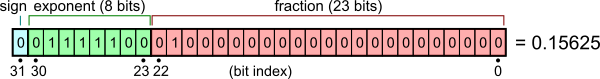
\includegraphics[scale=0.7]{images/ieee32.png}
  \caption[Caption for LOF]{IEEE-754 binary32 encoding\footnotemark}
\end{figure}
\footnotetext{IEEE-754 binary32 encoding:
  \url{https://en.wikipedia.org/wiki/Single-precision_floating-point_format}}

When parsing a {\tt binary32} we start by extracting all the relevant bits out
into separate numbers. We can then apply the following formula to get its
decimal value.

\begin{equation}
  value = (-1)^{sign} \cdot (1 + \sum^{23}_{i=1} frac_{23-i}2^{-i}) \cdot 2^{exp - 127}
\end{equation}

% type lattice

When performing arithmetic instruction on numbers, the machine enforces strong
typing and will therefore throw an exception if the operands is not of the same
type. This is to avoid common pitfalls, such as not handling overflow of
numbers, but also when doing arithmetic operations of two different types of
numbers. The compiler itself will have to truncate or convert values to matching
types before performing arithmetic operations.

Take, for instance, a program attempting to divide a floating-point precision
number by an integer number, will the result be an floating point or integer?
The only scenario where the machine itself needs to make a choice about is with
stack elements of type {\tt AnyType}. Instead of having a long list of what do
do in every case of all types, the choice will be defined by a type
lattice. This type lattice will control what type the result is of, in a given
operation between two numbers of different types.

All binary arithmetic operations follow the same type lattice. The type lattice
has the following set of rules matching which operand that is to be converted,
where the resulting conversion is also the type of the result.

\begin{itemize}
  \item If both operands is of the same type, nothing needs to be done.
  \item Otherwise, if either operand is a double floating-point precision
    number, the other operand is converted to a double also.
  \item Otherwise, if either operand is a single floating-point precision
    number, the other operand is converted to a float also.
  \item Otherwise, if either operand is of different signs, i.e. one is unsigned
    and the other is signed, the signed operand is converted to the an signed
    integer of the largest size of the two operands.
  \item Otherwise, the operands is of integer types of the same sign, where we
    return the largest of the two.
\end{itemize}

If none of the rules apply it will mean that at least one of the given operands
is of a type not supporting arithmetic operations. In this case, an exception
will be thrown.

If a type is converted to a type of smaller size, the value it truncated and has
a risk of overflowing, changing the value of the number. The {\tt noOverflow}
prefix defines if an exception should be thrown if overflow occurs.

\subsubsection{Fields}
\label{sec:implementation:meta:fields}

Fields are also a type of metadata, describing a member of a {\tt Composite}
type, in the form of field definition. It is important to note that fields are
not types themselves, like {\tt Composite} is, but a meta element describing a
field definition. Consequently, a field definition has a type element describing
the type of its content.

The internal data representation of a field definition, is as all other meta
types, an extension of the {\tt meta\_base} struct, giving it a type of meta, in
the form of a tag, and a unique hash. The field definition struct, {\tt
  meat\_field} extends this by adding a name, which is a index into the string
table, an integer offset, which is the distance where its value is stores from
the beginner of the heap object, and lastly a type describing its content. In
addition to these it a has an arbitrary number of properties and versions, which
are not implemented. The version element is to support dynamic languages
which can be extended or monkey patched, as Rubyists like to call it. Therefore,
a number of similar fields can exist in memory, which are distinguished by
version. % TODO

A field can be defined with set of properties, modifying its functionality. Such
properties are {\em abstract}, where the field is not actually initialized, only
declared. This is useful for languages with interfaces or abstract methods, akin
to Java's abstract classes and methods where another class can extend the
abstract class, implementing its already defined fields and methods.

Another property is {\em final}, where the the specific content of the field
cannot be changed. If the content is a reference, for instance, the referenced
value will always be the same, but the value of reference may still be mutated.

The last property is {\em strict layout}, where the value of the field is
guaranteed to be placed directly preceding to the field definition on the
heap. This enabled the compiler to the {\tt offset} element to reference the
content of the field. This is though considered unsafe, and thus the instruction
must be prefixed with the {\tt unsafe} flag.
%TODO afaik, fields har ikke strick layout, kun composites

\subsubsection{Sub-routines}
\label{sec:implementation:meta:sub-routines}

The last kind of metadata is a sub-routine which defines an executable set of
instructions. It is similar to a function (as in C), with the exception that a
sub-routine does not return a value. Rather, as described in
Section~\ref{sec:design:exec:sub-routine}, a sub-routine can modify values by
reference or by modifying stack elements upward into the stack, outside its own
stack frame.

A sub-routine defines a low-address which is the entry point of execution upon
invocation, and a high-address which is the the last instruction belonging to
it, together defining the address bounds of the sub-routine. Branching
instructions are not allowed to target addresses outside the bounds of the
currently executing sub-routine because it can be a security risk to execute
arbitrary code. This becomes an issue when linking multiple executables which
are ignorant of each others program data.

A special type of sub-routine is that defined by the run-time. Instead of using
a byte code address, they are currently hardcoded into the machine and are
invoked via a C function pointer. The run-time function is executed and then
execution continues as before, meaning that the semantics from the running
program's point of view are identical to that of usual sub-routines. The machine
distinguishes between run-time sub-routines and normal ones by their name;
language implementations are required to mangle the names of all symbols
(i.e.~field, sub-routines and type names) and prepend them with the ``\_''
characters. Upon invocation, if the name of the sub-routine does not start with
``\_'' then it is dispacted as a run-time function and if not the program
counter is changed to the sub-routines entry address.

The arguments that are accepted by a sub-routine are defined in its metadata
entry, but are currently not implemented. They would be used to verify that the
type of the elements currently on the stack align with the types of arguments,
and if not throw an exception.

%%% Local Variables:
%%% mode: latex
%%% TeX-master: "../report"
%%% End:


\subsection{Scopes}

Scopes are implemented as an array of key-value pairs that we call symbols, in
which the key is a string and the value is a function pointer. Obviously, the
value of a symbol should be an arbitrary type, as almost anything should be
storable in a symbol, but so far we have only used scopes to implement the
run-time library and thus have not made a generic symbol implementation. Name
resolution in a scope is carried out by iterating the array of symbols and
comparing names with the name that is being searched for. This is simple and
inefficient but sufficient for small test programs.

The obviously superior implementation would be a hash map, where a symbol's name
is hashed into an integer value and stored in an array indexed by the hashed
value of the name. This requires an array that is as large as the output of the
hash function which is likely to be unacceptable since most hash functions
compute at least 32-bit resulting in a 4.4 billion elements long array. Instead
the desired size of array is chosen, $n$, and the hash keys are computed
$\mod n$ to find the index. It is possible for two different names to have the
same $\mod$'d value, called a collision. To mitigate this each entry in the
array is a linked list of symbols that also stores the full hash value. As a
result, if a collision occurs it is possible to iterate the linked list and find
the symbol that matches the full hash.

\subsection{Instructions}
\label{sec:implementation:instr}
\subsubsection{Control Flow}
\label{sec:implementation:instr:control-flow}

At its core control flow is about changing the program counter of an executing
thread. The program counter, also known as the instruction pointer, is an
unsigned integral value representing an address in the byte code where the
machine will start parsing the next instruction. Instructions can change the
value of the program counter during execution which is the basis of all control
flow instructions, including branching and sub-routine calls.

The program counter is implemented as a field on the thread state and since the
thread state is the fundamental argument to all instruction functions, it is
trivial to change the program counter at any time. Because the byte code
programs are byte \textit{addressed} and most instructions span several bytes,
it is possible to set the program counter to a byte that is in the middle of an
instruction, which would lead to unpredictable unwanted behavior. Assemblers
usually use named labels that mark specific locations in assembly code and are
converted to actual addresses when assembled into binary format. It could also
be a task of the byte code verifier to assert that addresses always point to the
beginning of an instruction (as described in
Section~\ref{sec:separate-components:verifier:branch}).

Branching is the most fundamental control flow operation and is implemented
simply by setting the executing thread's program counter directly. Certain
checks are made to verify that a given address is a legal branch target.

Sub-routines are essentially implemented in the exact same way as branching
operations but with the addition of an activation element being pushed to the
stack. The activation element contains the address of the call site which is
used to set the program counter back when a return instruction is executed. In
addition to being on the stack, pointers to activation elements are saved as a
linked list in the thread state making it possible to retrieve its information
without having to search through the stack. Among others, it is used to check
whether the program counter is exceeding the address bounds of the current
sub-routine, which will result in an implicit return.

\subsubsection{Prefixes}

Instructions can be prefixed to modify the behavior of certain instructions.

Integer arguments to instruction are by default 8-bit integer values meaning
that a single code byte is consumes from the byte code stream. The {\tt large}
prefix extends this to 32-bits, i.e.~four bytes, which will likewise be consumed
and the program counter incremented accordingly.

The {\tt noOverflow} prefix signals the machine to throw exceptions if overflow
occurs when executing the following arithmetic instruction. Overflow is detected
differently for the various arithmetic operations and operand types. This is
required as different as types have different maximum and minimum values. We
will briefly explain the challenge of handling overflow in different scenarios
and how \thename{} currently, and imperfectly, tackles them.

Looking at how to detect overflow when doing arithmetic operations on {\em
  signed integer} operands, we have to take the size of the the operands' type
into account. For instance, an {\tt Int8} can only represent integer numbers in
the rage of -128 to 127. Knowing the type's maximum and minimum value, we can
deduce whether the operation will induce over- or underflow on operand $a$ and
$b$. In the case where the operation is addition, we check if operand $b$ is
larger than zero {\em and} operand $a$ is lesser than the sum of the type's
maximum value and $b$'s inverse. This can be denoted in the following formula:

\label{eq:overflow}
\begin{equation}
  overflow = (b > 0) \wedge (a > max - b)
\end{equation}

In a similar fashion we can detect underflow by:

\begin{equation}
  underflow = (b < 0) \wedge (a < min - b)
\end{equation}

If the operation is subtraction, we just change the plus operator to minus, in
the two equations. In the case of multiplication we use division, etc.

For unsigned integers the case is a little simpler, as the operand cannot be
negative. Therefore, when doing addition, underflow can per definition not
occur:

\begin{equation}
  a + b > 0, \qquad when\ a > 0, b > 0
\end{equation}

For substitution, we only needs to check if the $b$ operand is greater
than $a$, which will result in a negative number, thus inducing underflow.

\begin{equation}
  a - b < 0, \qquad when\ a > 0, b > a
\end{equation}

These fairly simple solutions has shown through tests, to work well where the
operand precision is not {\tt Int64} or {\tt UInt64}. The reason for this is
that all overflow check function promote each operand to an {\tt int64\_t} or
{\tt uint64\_t}, which prevents overflow of all operands with lower
precision. In the case of 64-bit integers, there is a risk of the check itself
to overflow. More precisely, $a < min - b$ will overflow if $b$ is
positive. There is not good solution for this, other than to use a higher
precision number for the tests. As C does not have any built-in data types of
larger precision, one would have to use multi-precision numbers which would
require some time to implement. We have chosen to note the short comings of the
current solution and focus our attention else where.

Both GCC and Clang has built-in functions for doing integer arithmetic while
also detecting
overflow\footnote{\url{https://gcc.gnu.org/onlinedocs/gcc/Integer-Overflow-Builtins.html}}\footnote{http://clang.llvm.org/docs/LanguageExtensions.html\#checked-arithmetic-builtins}. GCC's
implementation does this by converting the two operands into infinite precision
numbers, where after doing the the operation on the promoted operands. The
result is then cast to the original precision. If the casted result does not
equal the infinite precision result, overflow has occurred, which is indicated
by the functions return value. We have chosen to not use these to hold the
implementation as library independent as possible.

Detecting overflow for floating-point precision numbers is somewhat more
challenging, due to the more complex nature of its encoding. The C Standard
Library has built-in constants for finding a float's maximum value; {\tt
  FLT\_MIN} and {\tt FLT\_MAX} for single precision, {\tt DBL\_MIN} and {\tt
  DBL\_MAX} for double precision. These could in theory be used in the same
fashion as above, creating an efficient solution, given that we could do
built-in arithmetic operations on them. This is unfortunately not true, as {\tt
  FLT\_MAX - 1}, for instance, is regarded as undefined behavior and will on
most platforms be equal to {\tt FLT\_MAX}. Inducing undefined behavior when
trying to deduce whether an instruction is safe, renders its point
moot.

We have therefore chosen to use a simple but also sub-optimal solution. When,
for instance, adding two floats together that should produce overflow, the
resulting value will become equal to {\tt FLT\_MAX} (in the case of single
precision). We therefore check whether the result of each operation either
equals the maximum or minimum value for the given precision. In cases where an
operation equals exactly the maximum or minimum value, an overflow exception
will be thrown, even though under- or overflow might not have occurred.

\subsubsection{Arithmetic}

The arithmetic operations we have implemented is addition, substitution,
multiplication, division, remainder and negation. With the exception of the
latter, these are all binary operations, used through reverse-polish notation,
or suffix notation. We have made use of C's build in operators to make this as
efficient as possible. As the machine enforces strong typing, an exception will
be thrown if the operands are not of the same type. The only exception is if the
operand is of {\tt AnyType}, where it will automatically be converted to a
matching type.

Different types have to be handled differently to ensure correct
computations. For instance, an integer type cannot be used in the same way as a
floating-point number. To do this, we interpret the operands to its
corresponding C built-in type, perform the operation, and converting them back
to its standard machine type. We cannot rely on GCC to cast the types directly,
as this would be platform dependent; different platform use different endianness
and standards for storing number in memory.

These binary arithmetic operations are very similar in implementation, so we
have chosen to use C macros to keep the code base tidy, and not have to repeat
our selves. In summary this macro does the following:

\begin{enumerate}
  \item Ensure the top two stack elements are of the same type or {\tt AnyType}
  \item Pop them off the stack
  \item Align the types if either is {\tt AnyType}
  \item Allocate space for the result
  \item Decode the operands to their corresponding C type
  \item Perform the arithmetic operation
  \item If the {\tt noOverflow} prefix is set, check for overflow
  \item Encode result back to machine type
  \item Push the result onto the stack
\end{enumerate}

The saturated variants of the arithmetic instructions are implemented by
bounding the result of an arithmetic instruction within the range of the given
type.

As explained in Section~\ref{sec:design:stack:logic}, logical operations include
{\tt and}, {\tt or}, {\tt xor}, {\tt not}, left- and right-wise bit-shift ({\tt
  shl}, and {\tt shr}) and arithmetic right-wise bit-shift ({\tt ashr}). With
the exception of {\tt not}, their corresponding instructions are implemented in
a similar fashion as those of the arithmetic, through a macro using C's built-in
operators. The {\tt not} instruction takes a {\tt Boolean} value, which is
either {\tt 0x00} or {\tt 0x01}, and flips its value.

Lastly, we also have two sets of compare instructions, either comparing two
numeric operands of matching type or comparing a single numeric operand to zero
(or null). Each category includes equals, lesser-than and greater-than
instructions, all of which push a {\tt Boolean} result value onto the stack.

\subsubsection{Boxing}

% TODO: review
As explained in Section~\ref{sec:design:object-model}, all stacks are private to
the thread owning, making the only possible mechanism of sharing data to move
the data to the stack, i.e.~boxing it.

When trying to box a stack element trough the \instr{box} instruction, the top
element is popped off the stack and stored on the heap. An element with a
reference to the heap object is in turn pushed onto the stack. The type of the
new element will be a {\tt Reference<t>} type, where {\tt t} is the type of the
stack element which was boxed. If this type is not found in the meta table
already it is generated at run-time.

The \instr{unbox} instruction essentially does exactly the opposite, pushing the
referenced value to stack and asking telling the garbage collector that its
former heap object is not any longer used.


%%% Local Variables:
%%% mode: latex
%%% TeX-master: "../report"
%%% End:


\subsection{Run-Time Library}

The run-time library is implemented in the \code{runtime\_lib} module as a
collection of functions, one for each available run-time function. There are
currently two functions available namely \code{push\_scope} and \code{iprint}
which pushes a scope onto the current one and prints an integer value from the
stack, respectively.

% TODO: mention push scope as an example?

\subsection{Testing}
Throughout the project we have made heavy use of testing to ensure the
correctness of the implementation, i.e.~whether it strictly follows the machine
specification~\ref{sec:spec}. We have both made use of \term{unit}- and
\term{integration-tests}. Here unit-tests have the purpose of testing a single
isolated component, typically a single function. We mock a specific state of the
machine, or the state of a component in the machine, and then run isolated
functions where we {\it know} what the result should be, which can easily be
asserted. By comparison, the integration-tests have a much larger scope, in that
their purpose is to test the whole machine without any regard to any specific
component. This effectively ensures each component is wired together correctly.

For parts of the implementation we have made use of \term{test-driven
  development} (TDD). We write the tests prior to implementing the actual
functionality being tested. This eliminates the danger of false positives, where
tests pass when they are not supposed to. It also offers an efficient work flow,
where the minimum functionality is implemented to make the tests pass.
%TODO det har vi ikke sådan RIGTIG, evt w/e

\subsubsection{Unit-tests}

Unit-testing in C is a fairly simple process and essentially does not require
any framework or library. While not required, a simple set of \term{macros} will
greatly improve the readability and ease of writing tests.

% cmocka
In spite of this, we have chosen to use a unit-testing library called {\it
  Cmocka}\cite{cmocka}. It is a well tested and documented library, also used by
large projects like {\it libssh}~\footnote{Implementation of the SSH protocol:
  \url{http://libssh.org/}}. It offers several features which makes unit-testing
more powerful and simpler to write. For instance, it offers test suites and
\term{mocking} of objects which enabled us to set up a specific state of the
machine. With this state, we can run isolated tests, manipulating the state and
thereafter asserting that the correct transformations and output has occurred.

Cmocka also allows the test program to recover from signaled exceptions,
e.g. {\tt SIGSEGV}, {\tt SIGKILL}, etc. If a test in the test program triggers a
segmentation fault exception, for instance, it will not exit, but rather show
where the exception occurred and print useful debugging information like the
call stack.

Lastly, the library works on a wide range of platforms and only depends on the C
standard library. This makes it possible to use the library on embedded
platforms and with different compilers.

% example
As an example, we will describe how we test parts of the stack implementation.

Firstly, we create a mocked state of a stack which we can use for our tests.

%XXX assertions shouldn't happen in setup
\begin{lstlisting}[language={[ANSI]C},caption={Unit-test setup procedure}]
  static int setup(void **state)
  {
    stack_t *s = malloc(sizeof(stack_t));
    stack_init(s, 100);

    assert_non_null(s->elements);
    assert_int_equal(100, s->max_size);
    assert_int_equal(0, sum_stack(s));

    *state = s;

    return 0;
  }
\end{lstlisting}

In the above code listing, we initialize a stack object, do some simple
assertions, and store it in the {\tt state} variable passed with the setup
function. As we see below, this state is given as argument to all test cases
which easily allows us to retrieve it by dereferencing.

\begin{lstlisting}[language={[ANSI]C},caption={Unit-test of {\tt stack\_pop}}]
  static void test_pop(void **state)
  {
    stack_t *s = *state;

    uint32_t sum = sum_stack(s);

    stack_push(s, make_se_int(1));
    stack_push(s, make_se_int(2));
    stack_push(s, make_se_int(3));

    assert_int_equal(3, SE_INT(stack_pop(s)));
    assert_int_equal(2, SE_INT(stack_pop(s)));
    assert_int_equal(1, SE_INT(stack_pop(s)));

    assert_int_equal(sum, sum_stack(s));
  }
\end{lstlisting}

After having retrieved the stack for the {\tt state} parameter, we create an XOR
sum of the stack. When having tested the specific function, we assert that the
new XOR sum is the same as before, making sure that there is no unexpected
changes to the stack. Due to the simple nature of our {\tt stack\_sum} function,
this is not a guarantee, as different states of the stack may compute the same
sum, but will however catch most such problems.

In the body of a test case, the {\tt stack\_pop} function in this case, we push
several elements to the stack and assert that they are popped off again in the
correct order.

After all test cases has completed, a teardown function is run, reversing that
of the setup function. In the case of the stack tests, it simply frees the
memory allocated to the state of the stack.

\subsubsection{Integration-tests}

We want our integration tests to test the implementation in the fashion of
black-box testing, i.e.~given some input, the program should produce a specific
output, regardless of how the program works internally. The easiest way of
accomplishing this is by taking the actual machine executable and running it
with certain programs and arguments. We have therefor created several different
programs, from which we know the desired output.

As an example we can check that the machine fails when stack underflow occurs,
i.e.\ popping more values off the stack then there are actual values.

A valid test program for this would consist of a single instruction, \instr{POP,
  1}, producing a stack underflow error. We can test the output of the machine
by both asserting the exit code of the process, where we will have specified the
meanings of different exit codes, and by asserting what is written to standard
out and error ({\tt stdout} and {\tt stderr}). In the case of stack underflow
the exit code should be 4 and the output should match ``underflow'' (TODO:
update).

To automate this process we use shell scripting. For convenience, we have chosen
to utilize a shell testing framework, called shUnit2\footnote{shUnit2, unit
  testing for shell scripts: \url{http://code.google.com/p/shunit2/}}. This lets
us streamline the integration testing process, in contrast to manually running
each machine program and checking the output.

shUnit2 enables us to have an alias for the actual machine binary, letting us
set the target binary through our build system and piping standard error to
standard out. In our test cases we can then, by using the alias, store the
output and exit code in variables and do assertions based on their expected
values.
% TODO: update return code
\begin{lstlisting}[language={sh},caption={shUnit2 underflow test case}]
  test_stack_underflow()
  {
    output=$(am --file ${PDIR}/underflow.amb)
    ret=$?

    assertEquals "return code should be 4" 4 $ret
    assertTrue "output should include underflow" \
    "contains \"$output\" \"underflow\""
  }
\end{lstlisting}

In the above test case we run the machine with the underflow program, asserting
that the process exits with the correct code and that the output contains the
word `underflow`.


%%% Local Variables:
%%% mode: latex
%%% TeX-master: "../report"
%%% End:
